% Options for packages loaded elsewhere
\PassOptionsToPackage{unicode}{hyperref}
\PassOptionsToPackage{hyphens}{url}
%
\documentclass[
]{article}
\usepackage{lmodern}
\usepackage{amssymb,amsmath}
\usepackage{ifxetex,ifluatex}
\ifnum 0\ifxetex 1\fi\ifluatex 1\fi=0 % if pdftex
  \usepackage[T1]{fontenc}
  \usepackage[utf8]{inputenc}
  \usepackage{textcomp} % provide euro and other symbols
\else % if luatex or xetex
  \usepackage{unicode-math}
  \defaultfontfeatures{Scale=MatchLowercase}
  \defaultfontfeatures[\rmfamily]{Ligatures=TeX,Scale=1}
\fi
% Use upquote if available, for straight quotes in verbatim environments
\IfFileExists{upquote.sty}{\usepackage{upquote}}{}
\IfFileExists{microtype.sty}{% use microtype if available
  \usepackage[]{microtype}
  \UseMicrotypeSet[protrusion]{basicmath} % disable protrusion for tt fonts
}{}
\makeatletter
\@ifundefined{KOMAClassName}{% if non-KOMA class
  \IfFileExists{parskip.sty}{%
    \usepackage{parskip}
  }{% else
    \setlength{\parindent}{0pt}
    \setlength{\parskip}{6pt plus 2pt minus 1pt}}
}{% if KOMA class
  \KOMAoptions{parskip=half}}
\makeatother
\usepackage{xcolor}
\IfFileExists{xurl.sty}{\usepackage{xurl}}{} % add URL line breaks if available
\IfFileExists{bookmark.sty}{\usepackage{bookmark}}{\usepackage{hyperref}}
\hypersetup{
  pdftitle={Quantification of AMPK Knockout Blots},
  pdfauthor={Katherine Kistler and Dave Bridges},
  hidelinks,
  pdfcreator={LaTeX via pandoc}}
\urlstyle{same} % disable monospaced font for URLs
\usepackage[margin=1in]{geometry}
\usepackage{color}
\usepackage{fancyvrb}
\newcommand{\VerbBar}{|}
\newcommand{\VERB}{\Verb[commandchars=\\\{\}]}
\DefineVerbatimEnvironment{Highlighting}{Verbatim}{commandchars=\\\{\}}
% Add ',fontsize=\small' for more characters per line
\usepackage{framed}
\definecolor{shadecolor}{RGB}{248,248,248}
\newenvironment{Shaded}{\begin{snugshade}}{\end{snugshade}}
\newcommand{\AlertTok}[1]{\textcolor[rgb]{0.94,0.16,0.16}{#1}}
\newcommand{\AnnotationTok}[1]{\textcolor[rgb]{0.56,0.35,0.01}{\textbf{\textit{#1}}}}
\newcommand{\AttributeTok}[1]{\textcolor[rgb]{0.77,0.63,0.00}{#1}}
\newcommand{\BaseNTok}[1]{\textcolor[rgb]{0.00,0.00,0.81}{#1}}
\newcommand{\BuiltInTok}[1]{#1}
\newcommand{\CharTok}[1]{\textcolor[rgb]{0.31,0.60,0.02}{#1}}
\newcommand{\CommentTok}[1]{\textcolor[rgb]{0.56,0.35,0.01}{\textit{#1}}}
\newcommand{\CommentVarTok}[1]{\textcolor[rgb]{0.56,0.35,0.01}{\textbf{\textit{#1}}}}
\newcommand{\ConstantTok}[1]{\textcolor[rgb]{0.00,0.00,0.00}{#1}}
\newcommand{\ControlFlowTok}[1]{\textcolor[rgb]{0.13,0.29,0.53}{\textbf{#1}}}
\newcommand{\DataTypeTok}[1]{\textcolor[rgb]{0.13,0.29,0.53}{#1}}
\newcommand{\DecValTok}[1]{\textcolor[rgb]{0.00,0.00,0.81}{#1}}
\newcommand{\DocumentationTok}[1]{\textcolor[rgb]{0.56,0.35,0.01}{\textbf{\textit{#1}}}}
\newcommand{\ErrorTok}[1]{\textcolor[rgb]{0.64,0.00,0.00}{\textbf{#1}}}
\newcommand{\ExtensionTok}[1]{#1}
\newcommand{\FloatTok}[1]{\textcolor[rgb]{0.00,0.00,0.81}{#1}}
\newcommand{\FunctionTok}[1]{\textcolor[rgb]{0.00,0.00,0.00}{#1}}
\newcommand{\ImportTok}[1]{#1}
\newcommand{\InformationTok}[1]{\textcolor[rgb]{0.56,0.35,0.01}{\textbf{\textit{#1}}}}
\newcommand{\KeywordTok}[1]{\textcolor[rgb]{0.13,0.29,0.53}{\textbf{#1}}}
\newcommand{\NormalTok}[1]{#1}
\newcommand{\OperatorTok}[1]{\textcolor[rgb]{0.81,0.36,0.00}{\textbf{#1}}}
\newcommand{\OtherTok}[1]{\textcolor[rgb]{0.56,0.35,0.01}{#1}}
\newcommand{\PreprocessorTok}[1]{\textcolor[rgb]{0.56,0.35,0.01}{\textit{#1}}}
\newcommand{\RegionMarkerTok}[1]{#1}
\newcommand{\SpecialCharTok}[1]{\textcolor[rgb]{0.00,0.00,0.00}{#1}}
\newcommand{\SpecialStringTok}[1]{\textcolor[rgb]{0.31,0.60,0.02}{#1}}
\newcommand{\StringTok}[1]{\textcolor[rgb]{0.31,0.60,0.02}{#1}}
\newcommand{\VariableTok}[1]{\textcolor[rgb]{0.00,0.00,0.00}{#1}}
\newcommand{\VerbatimStringTok}[1]{\textcolor[rgb]{0.31,0.60,0.02}{#1}}
\newcommand{\WarningTok}[1]{\textcolor[rgb]{0.56,0.35,0.01}{\textbf{\textit{#1}}}}
\usepackage{longtable,booktabs}
% Correct order of tables after \paragraph or \subparagraph
\usepackage{etoolbox}
\makeatletter
\patchcmd\longtable{\par}{\if@noskipsec\mbox{}\fi\par}{}{}
\makeatother
% Allow footnotes in longtable head/foot
\IfFileExists{footnotehyper.sty}{\usepackage{footnotehyper}}{\usepackage{footnote}}
\makesavenoteenv{longtable}
\usepackage{graphicx}
\makeatletter
\def\maxwidth{\ifdim\Gin@nat@width>\linewidth\linewidth\else\Gin@nat@width\fi}
\def\maxheight{\ifdim\Gin@nat@height>\textheight\textheight\else\Gin@nat@height\fi}
\makeatother
% Scale images if necessary, so that they will not overflow the page
% margins by default, and it is still possible to overwrite the defaults
% using explicit options in \includegraphics[width, height, ...]{}
\setkeys{Gin}{width=\maxwidth,height=\maxheight,keepaspectratio}
% Set default figure placement to htbp
\makeatletter
\def\fps@figure{htbp}
\makeatother
\setlength{\emergencystretch}{3em} % prevent overfull lines
\providecommand{\tightlist}{%
  \setlength{\itemsep}{0pt}\setlength{\parskip}{0pt}}
\setcounter{secnumdepth}{5}

\title{Quantification of AMPK Knockout Blots}
\author{Katherine Kistler and Dave Bridges}
\date{June 18, 2020}

\begin{document}
\maketitle

{
\setcounter{tocdepth}{2}
\tableofcontents
}
\hypertarget{purpose}{%
\section{Purpose}\label{purpose}}

\hypertarget{experimental-details}{%
\section{Experimental Details}\label{experimental-details}}

Blotted liver lysates for AMPK and ACC

\hypertarget{raw-data}{%
\section{Raw Data}\label{raw-data}}

These data can be found in
\textbf{/Users/davebrid/Documents/GitHub/TissueSpecificTscKnockouts/Mouse
Data/Liver AMPK Ketogenic Diet/All Figures/Blots/Quantification} in
files named \textbf{Male ACC.xls} and \textbf{Male pACC.xls}. This
script was most recently updated on \textbf{Tue Aug 4 13:02:03 2020}.

\hypertarget{analysis}{%
\section{Analysis}\label{analysis}}

\hypertarget{lipogenic-proteins}{%
\section{Lipogenic Proteins}\label{lipogenic-proteins}}

\hypertarget{fatty-acid-synthase}{%
\subsection{Fatty Acid Synthase}\label{fatty-acid-synthase}}

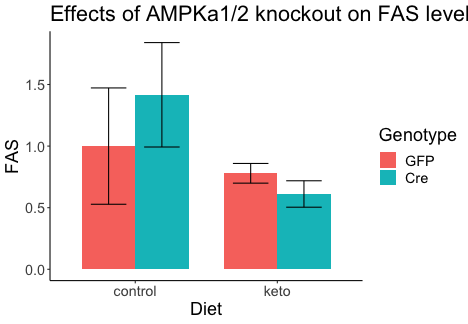
\includegraphics{figures/fas-barplot-1.png}

\begin{longtable}[]{@{}lrrrrr@{}}
\caption{ANOVA for FAS levels, no interaction}\tabularnewline
\toprule
term & df & sumsq & meansq & statistic & p.value\tabularnewline
\midrule
\endfirsthead
\toprule
term & df & sumsq & meansq & statistic & p.value\tabularnewline
\midrule
\endhead
Diet & 1 & 0 & 0 & 3.109 & 0.108\tabularnewline
Genotype & 1 & 0 & 0 & 0.123 & 0.733\tabularnewline
Residuals & 10 & 0 & 0 & NA & NA\tabularnewline
\bottomrule
\end{longtable}

\begin{longtable}[]{@{}lrrrrr@{}}
\caption{ANOVA for FAS levels, with interaction}\tabularnewline
\toprule
term & df & sumsq & meansq & statistic & p.value\tabularnewline
\midrule
\endfirsthead
\toprule
term & df & sumsq & meansq & statistic & p.value\tabularnewline
\midrule
\endhead
Diet & 1 & 0 & 0 & 3.093 & 0.113\tabularnewline
Genotype & 1 & 0 & 0 & 0.122 & 0.734\tabularnewline
Diet:Genotype & 1 & 0 & 0 & 0.949 & 0.356\tabularnewline
Residuals & 9 & 0 & 0 & NA & NA\tabularnewline
\bottomrule
\end{longtable}

\hypertarget{acetyl-coa-carboxylase}{%
\subsection{Acetyl-CoA Carboxylase}\label{acetyl-coa-carboxylase}}

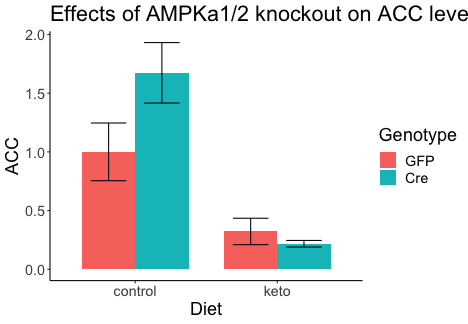
\includegraphics{figures/acc-barplot-1.png}

\begin{longtable}[]{@{}lrrrrr@{}}
\caption{ANOVA for ACC levels, no interaction}\tabularnewline
\toprule
term & df & sumsq & meansq & statistic & p.value\tabularnewline
\midrule
\endfirsthead
\toprule
term & df & sumsq & meansq & statistic & p.value\tabularnewline
\midrule
\endhead
Diet & 1 & 0 & 0 & 28.05 & 0.000\tabularnewline
Genotype & 1 & 0 & 0 & 1.62 & 0.232\tabularnewline
Residuals & 10 & 0 & 0 & NA & NA\tabularnewline
\bottomrule
\end{longtable}

\begin{longtable}[]{@{}lrrrrr@{}}
\caption{ANOVA for ACC levels, with interaction}\tabularnewline
\toprule
term & df & sumsq & meansq & statistic & p.value\tabularnewline
\midrule
\endfirsthead
\toprule
term & df & sumsq & meansq & statistic & p.value\tabularnewline
\midrule
\endhead
Diet & 1 & 0 & 0 & 39.70 & 0.000\tabularnewline
Genotype & 1 & 0 & 0 & 2.29 & 0.165\tabularnewline
Diet:Genotype & 1 & 0 & 0 & 5.15 & 0.049\tabularnewline
Residuals & 9 & 0 & 0 & NA & NA\tabularnewline
\bottomrule
\end{longtable}

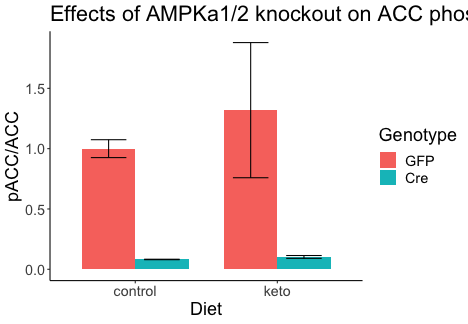
\includegraphics{figures/pACC-barplot-1.png}

\begin{longtable}[]{@{}lrrrrr@{}}
\caption{ANOVA for ACC phosphorylation, no interaction}\tabularnewline
\toprule
term & df & sumsq & meansq & statistic & p.value\tabularnewline
\midrule
\endfirsthead
\toprule
term & df & sumsq & meansq & statistic & p.value\tabularnewline
\midrule
\endhead
Diet & 1 & 0.305 & 0.305 & 0.112 & 0.744\tabularnewline
Genotype & 1 & 50.890 & 50.890 & 18.766 & 0.001\tabularnewline
Residuals & 10 & 27.118 & 2.712 & NA & NA\tabularnewline
\bottomrule
\end{longtable}

\begin{longtable}[]{@{}lrrrrr@{}}
\caption{ANOVA for ACC phosphorylation, with interaction}\tabularnewline
\toprule
term & df & sumsq & meansq & statistic & p.value\tabularnewline
\midrule
\endfirsthead
\toprule
term & df & sumsq & meansq & statistic & p.value\tabularnewline
\midrule
\endhead
Diet & 1 & 0.305 & 0.305 & 0.105 & 0.753\tabularnewline
Genotype & 1 & 50.890 & 50.890 & 17.515 & 0.002\tabularnewline
Diet:Genotype & 1 & 0.969 & 0.969 & 0.334 & 0.578\tabularnewline
Residuals & 9 & 26.149 & 2.905 & NA & NA\tabularnewline
\bottomrule
\end{longtable}

\hypertarget{s6-phosphorylation}{%
\subsection{S6 Phosphorylation}\label{s6-phosphorylation}}

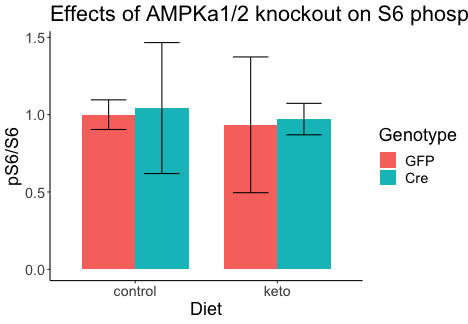
\includegraphics{figures/pS6-barplot-1.png}

\begin{longtable}[]{@{}lrrrrr@{}}
\caption{ANOVA for S6 phosphorylation, no interaction}\tabularnewline
\toprule
term & df & sumsq & meansq & statistic & p.value\tabularnewline
\midrule
\endfirsthead
\toprule
term & df & sumsq & meansq & statistic & p.value\tabularnewline
\midrule
\endhead
Diet & 1 & 0.726 & 0.726 & 0.058 & 0.815\tabularnewline
Genotype & 1 & 0.264 & 0.264 & 0.021 & 0.887\tabularnewline
Residuals & 10 & 125.354 & 12.535 & NA & NA\tabularnewline
\bottomrule
\end{longtable}

\begin{longtable}[]{@{}lrrrrr@{}}
\caption{ANOVA for S6 phosphorylation, with interaction}\tabularnewline
\toprule
term & df & sumsq & meansq & statistic & p.value\tabularnewline
\midrule
\endfirsthead
\toprule
term & df & sumsq & meansq & statistic & p.value\tabularnewline
\midrule
\endhead
Diet & 1 & 0.726 & 0.726 & 0.052 & 0.825\tabularnewline
Genotype & 1 & 0.264 & 0.264 & 0.019 & 0.893\tabularnewline
Diet:Genotype & 1 & 0.001 & 0.001 & 0.000 & 0.993\tabularnewline
Residuals & 9 & 125.353 & 13.928 & NA & NA\tabularnewline
\bottomrule
\end{longtable}

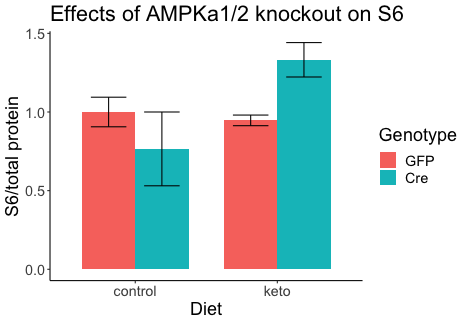
\includegraphics{figures/S6-barplot-1.png}

\begin{longtable}[]{@{}lrrrrr@{}}
\caption{ANOVA for S6, no interaction}\tabularnewline
\toprule
term & df & sumsq & meansq & statistic & p.value\tabularnewline
\midrule
\endfirsthead
\toprule
term & df & sumsq & meansq & statistic & p.value\tabularnewline
\midrule
\endhead
Diet & 1 & 0 & 0 & 3.101 & 0.109\tabularnewline
Genotype & 1 & 0 & 0 & 0.352 & 0.566\tabularnewline
Residuals & 10 & 0 & 0 & NA & NA\tabularnewline
\bottomrule
\end{longtable}

\begin{longtable}[]{@{}lrrrrr@{}}
\caption{ANOVA for S6, with interaction}\tabularnewline
\toprule
term & df & sumsq & meansq & statistic & p.value\tabularnewline
\midrule
\endfirsthead
\toprule
term & df & sumsq & meansq & statistic & p.value\tabularnewline
\midrule
\endhead
Diet & 1 & 0 & 0 & 4.398 & 0.065\tabularnewline
Genotype & 1 & 0 & 0 & 0.499 & 0.498\tabularnewline
Diet:Genotype & 1 & 0 & 0 & 5.182 & 0.049\tabularnewline
Residuals & 9 & 0 & 0 & NA & NA\tabularnewline
\bottomrule
\end{longtable}

\hypertarget{integrated-stress-response}{%
\section{Integrated Stress Response}\label{integrated-stress-response}}

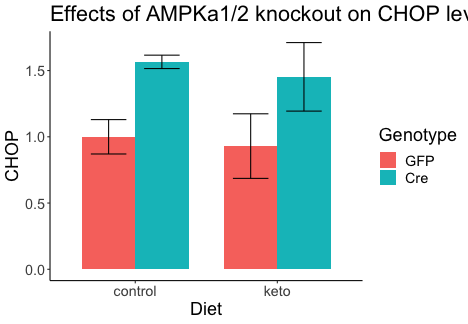
\includegraphics{figures/chop-barplot-1.png}

\begin{longtable}[]{@{}lrrrrr@{}}
\caption{ANOVA for CHOP levels, no interaction}\tabularnewline
\toprule
term & df & sumsq & meansq & statistic & p.value\tabularnewline
\midrule
\endfirsthead
\toprule
term & df & sumsq & meansq & statistic & p.value\tabularnewline
\midrule
\endhead
Diet & 1 & 0 & 0 & 0.075 & 0.790\tabularnewline
Genotype & 1 & 0 & 0 & 7.416 & 0.021\tabularnewline
Residuals & 10 & 0 & 0 & NA & NA\tabularnewline
\bottomrule
\end{longtable}

\begin{longtable}[]{@{}lrrrrr@{}}
\caption{ANOVA for CHOP levels, with interaction}\tabularnewline
\toprule
term & df & sumsq & meansq & statistic & p.value\tabularnewline
\midrule
\endfirsthead
\toprule
term & df & sumsq & meansq & statistic & p.value\tabularnewline
\midrule
\endhead
Diet & 1 & 0 & 0 & 0.067 & 0.801\tabularnewline
Genotype & 1 & 0 & 0 & 6.682 & 0.029\tabularnewline
Diet:Genotype & 1 & 0 & 0 & 0.010 & 0.921\tabularnewline
Residuals & 9 & 0 & 0 & NA & NA\tabularnewline
\bottomrule
\end{longtable}

\hypertarget{amp-activated-protein-kinase}{%
\subsection{AMP Activated Protein
Kinase}\label{amp-activated-protein-kinase}}

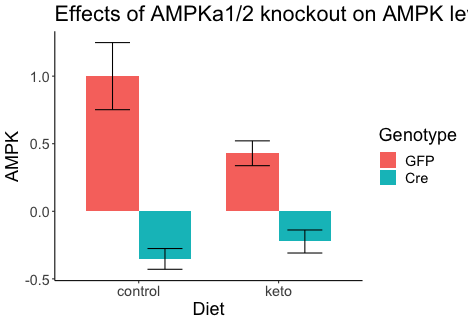
\includegraphics{figures/AMPK-barplot-1.png}

\begin{longtable}[]{@{}lrrrrr@{}}
\caption{ANOVA for AMPK levels, no interaction}\tabularnewline
\toprule
term & df & sumsq & meansq & statistic & p.value\tabularnewline
\midrule
\endfirsthead
\toprule
term & df & sumsq & meansq & statistic & p.value\tabularnewline
\midrule
\endhead
Diet & 1 & 0 & 0 & 2.48 & 0.147\tabularnewline
Genotype & 1 & 0 & 0 & 32.99 & 0.000\tabularnewline
Residuals & 10 & 0 & 0 & NA & NA\tabularnewline
\bottomrule
\end{longtable}

\begin{longtable}[]{@{}lrrrrr@{}}
\caption{ANOVA for AMPK levels, with interaction}\tabularnewline
\toprule
term & df & sumsq & meansq & statistic & p.value\tabularnewline
\midrule
\endfirsthead
\toprule
term & df & sumsq & meansq & statistic & p.value\tabularnewline
\midrule
\endhead
Diet & 1 & 0 & 0 & 3.83 & 0.082\tabularnewline
Genotype & 1 & 0 & 0 & 51.11 & 0.000\tabularnewline
Diet:Genotype & 1 & 0 & 0 & 6.49 & 0.031\tabularnewline
Residuals & 9 & 0 & 0 & NA & NA\tabularnewline
\bottomrule
\end{longtable}

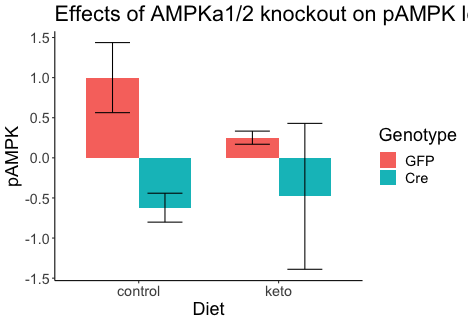
\includegraphics{figures/pAMPK-barplot-1.png}

\begin{longtable}[]{@{}lrrrrr@{}}
\caption{ANOVA for pAMPK levels, no interaction}\tabularnewline
\toprule
term & df & sumsq & meansq & statistic & p.value\tabularnewline
\midrule
\endfirsthead
\toprule
term & df & sumsq & meansq & statistic & p.value\tabularnewline
\midrule
\endhead
Diet & 1 & 0.179 & 0.179 & 0.343 & 0.571\tabularnewline
Genotype & 1 & 1.852 & 1.852 & 3.538 & 0.089\tabularnewline
Residuals & 10 & 5.235 & 0.524 & NA & NA\tabularnewline
\bottomrule
\end{longtable}

\begin{longtable}[]{@{}lrrrrr@{}}
\caption{ANOVA for pAMPK levels, with interaction}\tabularnewline
\toprule
term & df & sumsq & meansq & statistic & p.value\tabularnewline
\midrule
\endfirsthead
\toprule
term & df & sumsq & meansq & statistic & p.value\tabularnewline
\midrule
\endhead
Diet & 1 & 0.179 & 0.179 & 0.326 & 0.582\tabularnewline
Genotype & 1 & 1.852 & 1.852 & 3.363 & 0.100\tabularnewline
Diet:Genotype & 1 & 0.278 & 0.278 & 0.505 & 0.496\tabularnewline
Residuals & 9 & 4.957 & 0.551 & NA & NA\tabularnewline
\bottomrule
\end{longtable}

\hypertarget{atp-citrate-lyase}{%
\subsection{ATP citrate lyase}\label{atp-citrate-lyase}}

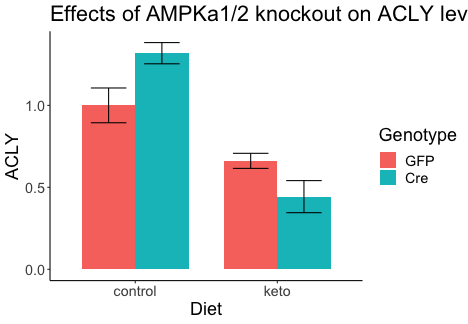
\includegraphics{figures/ACLY-barplot-1.png}

\begin{longtable}[]{@{}lrrrrr@{}}
\caption{ANOVA for ACLY levels, no interaction}\tabularnewline
\toprule
term & df & sumsq & meansq & statistic & p.value\tabularnewline
\midrule
\endfirsthead
\toprule
term & df & sumsq & meansq & statistic & p.value\tabularnewline
\midrule
\endhead
Diet & 1 & 0 & 0 & 27.777 & 0.000\tabularnewline
Genotype & 1 & 0 & 0 & 0.073 & 0.792\tabularnewline
Residuals & 10 & 0 & 0 & NA & NA\tabularnewline
\bottomrule
\end{longtable}

\begin{longtable}[]{@{}lrrrrr@{}}
\caption{ANOVA for ACLY levels, with interaction}\tabularnewline
\toprule
term & df & sumsq & meansq & statistic & p.value\tabularnewline
\midrule
\endfirsthead
\toprule
term & df & sumsq & meansq & statistic & p.value\tabularnewline
\midrule
\endhead
Diet & 1 & 0 & 0 & 51.166 & 0.000\tabularnewline
Genotype & 1 & 0 & 0 & 0.135 & 0.722\tabularnewline
Diet:Genotype & 1 & 0 & 0 & 9.420 & 0.013\tabularnewline
Residuals & 9 & 0 & 0 & NA & NA\tabularnewline
\bottomrule
\end{longtable}

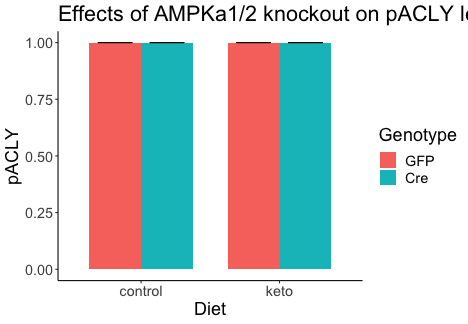
\includegraphics{figures/pACLY-barplot-1.png}

\begin{longtable}[]{@{}lrrrrr@{}}
\caption{ANOVA for pACLY levels, no interaction}\tabularnewline
\toprule
term & df & sumsq & meansq & statistic & p.value\tabularnewline
\midrule
\endfirsthead
\toprule
term & df & sumsq & meansq & statistic & p.value\tabularnewline
\midrule
\endhead
Diet & 1 & 0 & 0 & NaN & NaN\tabularnewline
Genotype & 1 & 0 & 0 & NaN & NaN\tabularnewline
Residuals & 10 & 0 & 0 & NA & NA\tabularnewline
\bottomrule
\end{longtable}

\begin{longtable}[]{@{}lrrrrr@{}}
\caption{ANOVA for pACLY levels, with interaction}\tabularnewline
\toprule
term & df & sumsq & meansq & statistic & p.value\tabularnewline
\midrule
\endfirsthead
\toprule
term & df & sumsq & meansq & statistic & p.value\tabularnewline
\midrule
\endhead
Diet & 1 & 0 & 0 & NaN & NaN\tabularnewline
Genotype & 1 & 0 & 0 & NaN & NaN\tabularnewline
Diet:Genotype & 1 & 0 & 0 & NaN & NaN\tabularnewline
Residuals & 9 & 0 & 0 & NA & NA\tabularnewline
\bottomrule
\end{longtable}

\hypertarget{mitochondria-complexes-band-1}{%
\subsection{Mitochondria Complexes Band
1}\label{mitochondria-complexes-band-1}}

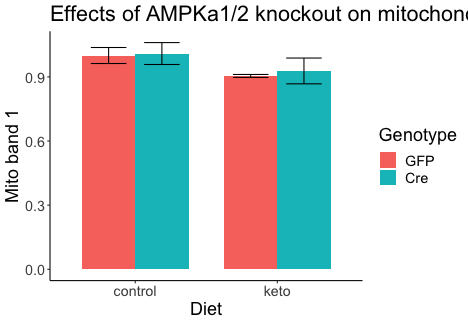
\includegraphics{figures/mitoband1-barplot-1.png}

\begin{longtable}[]{@{}lrrrrr@{}}
\caption{ANOVA for mitochondira band 1 levels, no
interaction}\tabularnewline
\toprule
term & df & sumsq & meansq & statistic & p.value\tabularnewline
\midrule
\endfirsthead
\toprule
term & df & sumsq & meansq & statistic & p.value\tabularnewline
\midrule
\endhead
Diet & 1 & 0 & 0 & 3.563 & 0.088\tabularnewline
Genotype & 1 & 0 & 0 & 0.132 & 0.724\tabularnewline
Residuals & 10 & 0 & 0 & NA & NA\tabularnewline
\bottomrule
\end{longtable}

\begin{longtable}[]{@{}lrrrrr@{}}
\caption{ANOVA for mitochondira band 1 levels, with
interaction}\tabularnewline
\toprule
term & df & sumsq & meansq & statistic & p.value\tabularnewline
\midrule
\endfirsthead
\toprule
term & df & sumsq & meansq & statistic & p.value\tabularnewline
\midrule
\endhead
Diet & 1 & 0 & 0 & 3.214 & 0.107\tabularnewline
Genotype & 1 & 0 & 0 & 0.119 & 0.738\tabularnewline
Diet:Genotype & 1 & 0 & 0 & 0.021 & 0.887\tabularnewline
Residuals & 9 & 0 & 0 & NA & NA\tabularnewline
\bottomrule
\end{longtable}

\hypertarget{mitochondira-complexes-band-2}{%
\subsection{Mitochondira Complexes band
2}\label{mitochondira-complexes-band-2}}

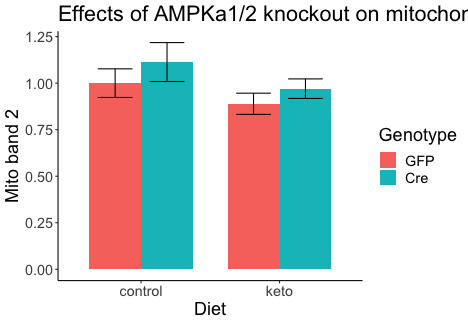
\includegraphics{figures/mitoband2-barplot-1.png}

\begin{longtable}[]{@{}lrrrrr@{}}
\caption{ANOVA for mitochondira band 2 levels, no
interaction}\tabularnewline
\toprule
term & df & sumsq & meansq & statistic & p.value\tabularnewline
\midrule
\endfirsthead
\toprule
term & df & sumsq & meansq & statistic & p.value\tabularnewline
\midrule
\endhead
Diet & 1 & 0 & 0 & 3.07 & 0.110\tabularnewline
Genotype & 1 & 0 & 0 & 1.92 & 0.196\tabularnewline
Residuals & 10 & 0 & 0 & NA & NA\tabularnewline
\bottomrule
\end{longtable}

\begin{longtable}[]{@{}lrrrrr@{}}
\caption{ANOVA for mitochondira band 2 levels, with
interaction}\tabularnewline
\toprule
term & df & sumsq & meansq & statistic & p.value\tabularnewline
\midrule
\endfirsthead
\toprule
term & df & sumsq & meansq & statistic & p.value\tabularnewline
\midrule
\endhead
Diet & 1 & 0 & 0 & 2.777 & 0.13\tabularnewline
Genotype & 1 & 0 & 0 & 1.741 & 0.22\tabularnewline
Diet:Genotype & 1 & 0 & 0 & 0.049 & 0.83\tabularnewline
Residuals & 9 & 0 & 0 & NA & NA\tabularnewline
\bottomrule
\end{longtable}

\hypertarget{mitochondria-complexes-band-3}{%
\subsection{Mitochondria Complexes Band
3}\label{mitochondria-complexes-band-3}}

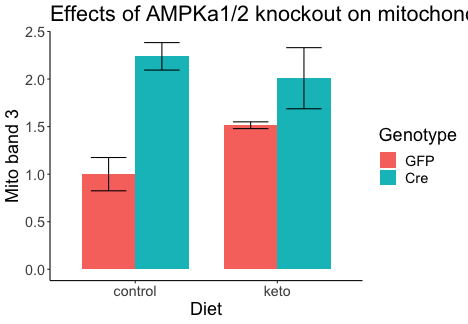
\includegraphics{figures/mitoband3-barplot-1.png}

\begin{longtable}[]{@{}lrrrrr@{}}
\caption{ANOVA for mitochondira band 3 levels, no
interaction}\tabularnewline
\toprule
term & df & sumsq & meansq & statistic & p.value\tabularnewline
\midrule
\endfirsthead
\toprule
term & df & sumsq & meansq & statistic & p.value\tabularnewline
\midrule
\endhead
Diet & 1 & 0 & 0 & 0.509 & 0.492\tabularnewline
Genotype & 1 & 0 & 0 & 11.392 & 0.007\tabularnewline
Residuals & 10 & 0 & 0 & NA & NA\tabularnewline
\bottomrule
\end{longtable}

\begin{longtable}[]{@{}lrrrrr@{}}
\caption{ANOVA for mitochondira band 3 levels, with
interaction}\tabularnewline
\toprule
term & df & sumsq & meansq & statistic & p.value\tabularnewline
\midrule
\endfirsthead
\toprule
term & df & sumsq & meansq & statistic & p.value\tabularnewline
\midrule
\endhead
Diet & 1 & 0 & 0 & 0.589 & 0.462\tabularnewline
Genotype & 1 & 0 & 0 & 13.175 & 0.005\tabularnewline
Diet:Genotype & 1 & 0 & 0 & 2.565 & 0.144\tabularnewline
Residuals & 9 & 0 & 0 & NA & NA\tabularnewline
\bottomrule
\end{longtable}

\hypertarget{mitochondira-complexes-band-4}{%
\subsection{Mitochondira Complexes Band
4}\label{mitochondira-complexes-band-4}}

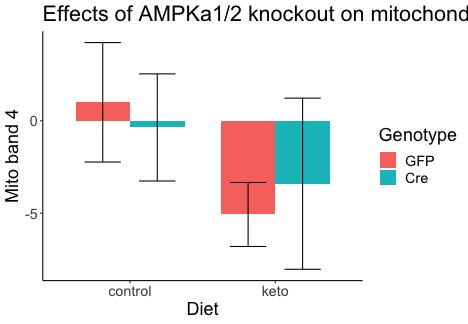
\includegraphics{figures/mitoband4-barplot-1.png}

\begin{longtable}[]{@{}lrrrrr@{}}
\caption{ANOVA for mitochondira band 4 levels, no
interaction}\tabularnewline
\toprule
term & df & sumsq & meansq & statistic & p.value\tabularnewline
\midrule
\endfirsthead
\toprule
term & df & sumsq & meansq & statistic & p.value\tabularnewline
\midrule
\endhead
Diet & 1 & 0 & 0 & 1.608 & 0.233\tabularnewline
Genotype & 1 & 0 & 0 & 0.005 & 0.944\tabularnewline
Residuals & 10 & 0 & 0 & NA & NA\tabularnewline
\bottomrule
\end{longtable}

\begin{longtable}[]{@{}lrrrrr@{}}
\caption{ANOVA for mitochondira band 4 levels, with
interaction}\tabularnewline
\toprule
term & df & sumsq & meansq & statistic & p.value\tabularnewline
\midrule
\endfirsthead
\toprule
term & df & sumsq & meansq & statistic & p.value\tabularnewline
\midrule
\endhead
Diet & 1 & 0 & 0 & 1.475 & 0.255\tabularnewline
Genotype & 1 & 0 & 0 & 0.005 & 0.946\tabularnewline
Diet:Genotype & 1 & 0 & 0 & 0.170 & 0.690\tabularnewline
Residuals & 9 & 0 & 0 & NA & NA\tabularnewline
\bottomrule
\end{longtable}

\hypertarget{mitochondria-complexes-band-5}{%
\subsection{Mitochondria Complexes Band
5}\label{mitochondria-complexes-band-5}}

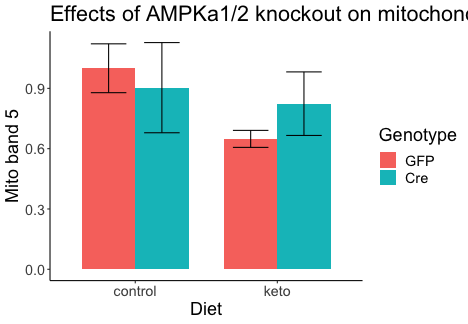
\includegraphics{figures/mitoband5-barplot-1.png}

\begin{longtable}[]{@{}lrrrrr@{}}
\caption{ANOVA for mitochondira band 5 levels, no
interaction}\tabularnewline
\toprule
term & df & sumsq & meansq & statistic & p.value\tabularnewline
\midrule
\endfirsthead
\toprule
term & df & sumsq & meansq & statistic & p.value\tabularnewline
\midrule
\endhead
Diet & 1 & 0 & 0 & 1.751 & 0.215\tabularnewline
Genotype & 1 & 0 & 0 & 0.099 & 0.760\tabularnewline
Residuals & 10 & 0 & 0 & NA & NA\tabularnewline
\bottomrule
\end{longtable}

\begin{longtable}[]{@{}lrrrrr@{}}
\caption{ANOVA for mitochondira band 5 levels, with
interaction}\tabularnewline
\toprule
term & df & sumsq & meansq & statistic & p.value\tabularnewline
\midrule
\endfirsthead
\toprule
term & df & sumsq & meansq & statistic & p.value\tabularnewline
\midrule
\endhead
Diet & 1 & 0 & 0 & 1.708 & 0.224\tabularnewline
Genotype & 1 & 0 & 0 & 0.096 & 0.763\tabularnewline
Diet:Genotype & 1 & 0 & 0 & 0.759 & 0.406\tabularnewline
Residuals & 9 & 0 & 0 & NA & NA\tabularnewline
\bottomrule
\end{longtable}

\hypertarget{session-information}{%
\section{Session Information}\label{session-information}}

\begin{Shaded}
\begin{Highlighting}[]
\KeywordTok{sessionInfo}\NormalTok{()}
\end{Highlighting}
\end{Shaded}

\begin{verbatim}
## R version 4.0.2 (2020-06-22)
## Platform: x86_64-apple-darwin17.0 (64-bit)
## Running under: macOS Catalina 10.15.5
## 
## Matrix products: default
## BLAS:   /Library/Frameworks/R.framework/Versions/4.0/Resources/lib/libRblas.dylib
## LAPACK: /Library/Frameworks/R.framework/Versions/4.0/Resources/lib/libRlapack.dylib
## 
## locale:
## [1] en_US.UTF-8/en_US.UTF-8/en_US.UTF-8/C/en_US.UTF-8/en_US.UTF-8
## 
## attached base packages:
## [1] stats     graphics  grDevices utils     datasets  methods   base     
## 
## other attached packages:
## [1] broom_0.5.6   ggplot2_3.3.2 readxl_1.3.1  dplyr_1.0.0   tidyr_1.1.0  
## [6] knitr_1.29   
## 
## loaded via a namespace (and not attached):
##  [1] Rcpp_1.0.5       highr_0.8        plyr_1.8.6       pillar_1.4.4    
##  [5] compiler_4.0.2   cellranger_1.1.0 tools_4.0.2      digest_0.6.25   
##  [9] evaluate_0.14    lifecycle_0.2.0  tibble_3.0.2     gtable_0.3.0    
## [13] nlme_3.1-148     lattice_0.20-41  pkgconfig_2.0.3  rlang_0.4.6     
## [17] yaml_2.2.1       xfun_0.15        withr_2.2.0      stringr_1.4.0   
## [21] generics_0.0.2   vctrs_0.3.1      grid_4.0.2       tidyselect_1.1.0
## [25] glue_1.4.1       R6_2.4.1         rmarkdown_2.3    purrr_0.3.4     
## [29] farver_2.0.3     magrittr_1.5     scales_1.1.1     backports_1.1.8 
## [33] ellipsis_0.3.1   htmltools_0.5.0  colorspace_1.4-1 labeling_0.3    
## [37] stringi_1.4.6    munsell_0.5.0    crayon_1.3.4
\end{verbatim}

\end{document}
